\documentclass[tikz,border=8pt]{standalone}
\usepackage{amsmath}\usepackage{pgfplots}\pgfplotsset{compat=1.18}\usetikzlibrary{arrows.meta}
\definecolor{ink}{HTML}{334155}\definecolor{blue}{HTML}{6366F1}\definecolor{green}{HTML}{059669}\definecolor{orange}{HTML}{EA580C}
\begin{document}
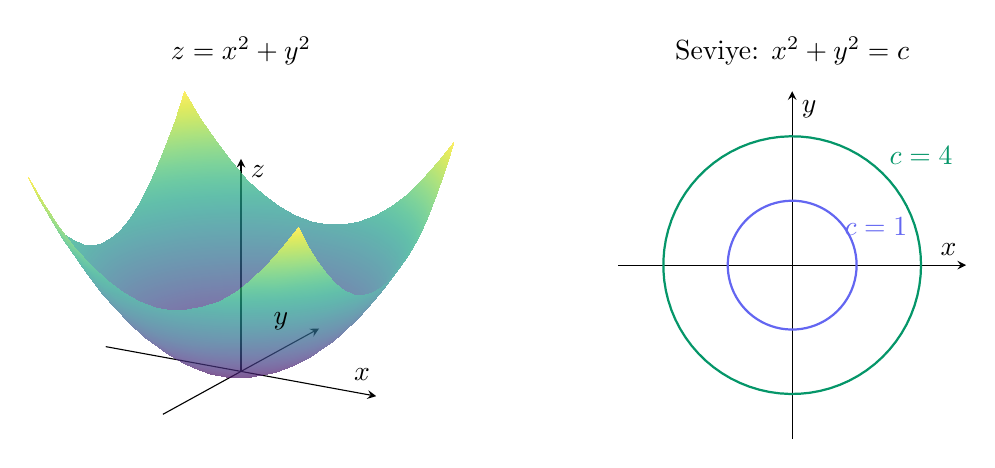
\begin{tikzpicture}
\begin{axis}[width=7cm,height=6cm,view={30}{25},axis lines=center,xlabel=$x$,ylabel=$y$,zlabel=$z$,ticks=none,title={$z=x^2+y^2$}]
\addplot3[surf,opacity=.7,shader=interp,domain=-2:2,y domain=-2:2,samples=18,colormap/viridis]{x^2+y^2};\end{axis}
\begin{axis}[at={(7.5cm,0)},anchor=south west,width=7cm,height=6cm,axis equal image,axis lines=middle,xmin=-2.7,xmax=2.7,ymin=-2.7,ymax=2.7,xlabel=$x$,ylabel=$y$,ticks=none,title={Seviye: $x^2+y^2=c$}]
\addplot[blue,thick,domain=0:360,samples=80]({cos(x)},{sin(x)});\addplot[green,thick,domain=0:360,samples=80]({2*cos(x)},{2*sin(x)});
\node[blue]at(axis cs:1.3,.6){$c=1$};\node[green]at(axis cs:2,1.7){$c=4$};\end{axis}\end{tikzpicture}
\end{document}
